\section{Εισαγωγή}
Τα δένδρα όπως και τα γραφήματα είναι μη γραμμικές δομές δεδομένων που αποτελούν συλλογές κόμβων. Τα δένδρα επιτρέπουν ιεραρχική οργάνωση των δεδομένων όπως φαίνεται στο Σχήμα \ref{fig:binary_tree}. Αυτό το στοιχείο τους επιτρέπει να έχουν καλύτερες επιδόσεις προσπέλασης των επιμέρους στοιχείων σε σχέση με τις γραμμικές λίστες. Με κατάλληλη διευθέτηση των στοιχείων ενός δένδρου καθώς και με εφαρμογή προχωρημένων μηχανισμών εισαγωγής και διαγραφής στοιχείων ο χρόνος εκτέλεσης των περισσότερων λειτουργιών σε ένα δένδρο (ισοζυγισμένο δυαδικό δένδρο αναζήτησης) γίνεται $O(\log n)$. Στην STL τα δένδρα χρησιμοποιούνται στην υλοποίηση των containers std::map και std::set.

\begin{figure}[htbp]
  \centering
  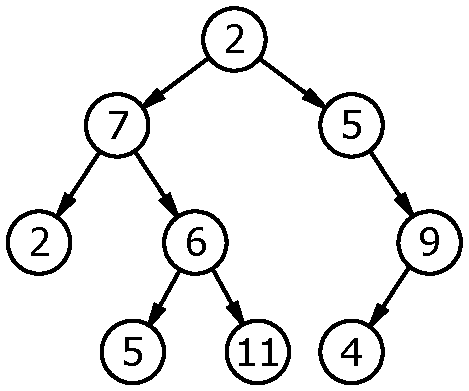
\includegraphics[width=80mm]{Binary_tree.pdf}
  \caption{Ένα απλό δένδρο \cite{wikipedia_binary_tree}}
  \label{fig:binary_tree}
\end{figure}

\section{Δένδρα}

Ένα δένδρο (tree) αποτελείται από κόμβους (nodes) που συνδέονται μεταξύ τους με κατευθυνόμενες ακμές (edges). Ο πρώτος (υψηλότερος) κόμβος του δένδρου ονομάζεται ρίζα (root) ενώ οι κόμβοι που βρίσκονται στα άκρα του δένδρου λέγονται φύλλα (leaves). Οι κόμβοι με τους οποίους συνδέεται απευθείας ένας κόμβος ονομάζονται παιδιά (children) του κόμβου. Αντίστοιχα, ένας κόμβος που έχει παιδιά ονομάζεται γονέας (parent) των αντίστοιχων παιδιών-κόμβων. Απόγονοι (descendants) ενός κόμβου είναι οι κόμβοι για τους οποίους υπάρχει διαδρομή-μονοπάτι (path) πραγματοποιώντας διαδοχικές μεταβάσεις από γονείς σε παιδιά. Αντίστοιχα ορίζεται και η έννοια των προγόνων (ancestors) ενός κόμβου με τη ρίζα να είναι ο μοναδικός κόμβος που δεν έχει προγόνους. 

Τα δένδρα είναι αναδρομικές δομές από τη φύση τους. Κάθε κόμβος ενός δένδρου ορίζει έναν αριθμό από μικρότερα δένδρα, ένα για κάθε παιδί του. Σε ένα δένδρο με $N$ κόμβους υπάρχουν πάντα $N-1$ ακμές καθώς όλοι οι κόμβοι εκτός από τον κόμβο ρίζα έχουν μια ακμή η οποία τους συνδέει με τον γονέα τους.

Το μήκος ενός μονοπατιού ανάμεσα σε δύο κόμβους είναι ίσο με το πλήθος των ακμών του μονοπατιού. Εφόσον υπάρχει μονοπάτι μέσω του οποίου συνδέονται δύο κόμβοι το μονοπάτι αυτό είναι μοναδικό. Για κάθε κόμβο ορίζεται ως \textbf{βάθος του κόμβου} (depth) το μήκος του μονοπατιού από τη ρίζα του δένδρου μέχρι τον ίδιο τον κόμβο. Αντίστοιχα, \textbf{ύψος ενός κόμβου} (height) είναι το μήκος του μακρύτερου μονοπατιού από τον κόμβο προς ένα από τα φύλλα του δένδρου για τα οποία υφίσταται μονοπάτι με αφετηρία τον κόμβο.


\section{Δυαδικά δένδρα}

Δυαδικό δένδρο είναι ένα δένδρο για το οποίο ισχύει ότι κάθε κόμβος έχει το πολύ δύο παιδιά \cite{parlante_binary_tree}. Ένα δένδρο μπορεί να διανυθεί με διαφορετικούς τρόπους. Ορισμένοι βασικοί τρόποι διάσχισης (traversal) του δένδρου παρουσιάζονται στη συνέχεια \cite{g4g_traversals}.

\subsection{Αναζήτηση κατά βάθος}

Η αναζήτηση κατά βάθος (DFS = Depth First Search) διανύει το δένδρο αναζήτησης εξαντλώντας μονοπάτια από τη ρίζα προς τα φύλλα του δένδρου. Ένας τρόπος για να επιτευχθεί αυτό είναι η χρήση αναδρομής. 

\subsubsection{Προ-διατακτική αναζήτηση κατά βάθος}

Στη διάσχιση του δένδρου προ-διατακτικά (pre-order) πρώτα πραγματοποιείται η επίσκεψη στη ρίζα και μετά καλείται αναδρομικά η ίδια συνάρτηση πρώτα για το αριστερό υποδένδρο και μετά για το δεξιό υποδένδρο. 
Συνηθισμένες χρήσεις της pre-order διάσχισης είναι η δημιουργία αντιγράφων ενός δένδρου καθώς και η λήψη της prefix μορφής ενός expression tree \cite{wikipedia_polish_notation}.

\subsubsection{Ένδο-διατακτική αναζήτηση κατά βάθος}

Στη διάσχιση του δένδρου ένδο-διατακτικά (in-order) καλείται αναδρομικά η συνάρτηση για το αριστερό υποδένδρο, μετά πραγματοποιείται επίσκεψη στη ρίζα και μετά καλείται αναδρομικά η συνάρτηση για το δεξιό υποδένδρο.
Εφόσον το δένδρο είναι δυαδικό δένδρο αναζήτησης, η in-order διάσχιση επιστρέφει τους κόμβους σε μη φθίνουσα σειρά. Σχετικά με το τι είναι τα δυαδικά δένδρα αναζήτησης δείτε την παράγραφο~\ref{bst}).

\subsubsection{Μέτα-διατακτική αναζήτηση κατά βάθος}

Στη διάσχιση του δένδρου μέτα-διατακτικά (post-order) πρώτα καλείται αναδρομικά η  συνάρτηση για το αριστερό υποδένδρο, μετά καλείται αναδρομικά για το δεξιό υποδένδρο και τέλος πραγματοποιείται η επίσκεψη στη ρίζα. 
Συνηθισμένες χρήσεις της post-order διάσχισης είναι η διαγραφή ενός δένδρου καθώς και η λήψη της postfix μορφής ενός expression tree \cite{wikipedia_reverse_polish_notation}.

\subsection{Αναζήτηση κατά πλάτος}

Στην αναζήτηση κατά πλάτος (BFS=Breadth First Search) οι κόμβοι του δένδρου διανύονται κατά επίπεδα ξεκινώντας από τη ρίζα και μεταβαίνοντας από πάνω προς τα κάτω. Σε κάθε επίπεδο η προσπέλαση στους κόμβους γίνεται από αριστερά προς τα δεξιά. Για να επιτευχθεί αυτό το είδος διάσχισης του δένδρου χρησιμοποιείται μια ουρά (queue) στην οποία μόλις εξετάζεται ένα στοιχείο προστίθενται στο πίσω άκρο της ουράς τα παιδιά του.

\lstinputlisting[caption = header file για το δυαδικό δένδρο (binary\_tree.hpp)]{lab09/binary_tree.hpp}

\lstinputlisting[caption = source file για το δυαδικό δένδρο αναζήτησης (binary\_tree.cpp)]{lab09/binary_tree.cpp}

Ο ακόλουθος κώδικας δημιουργεί το δυαδικό δένδρο του Σχήματος~\ref{fig:binary_tree1}.

\begin{figure}[htbp]
  \centering
  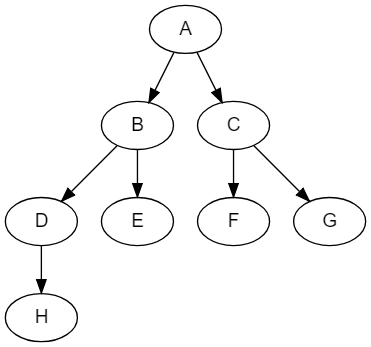
\includegraphics[width=80mm]{binary_tree1.png}
  \caption{Δυαδικό δένδρο με λεκτικά ως τιμές κλειδιών στους κόμβους}
  \label{fig:binary_tree1}
\end{figure}

\lstinputlisting[caption = Δοκιμή των συναρτήσεων του δυαδικού δένδρου (binary\_tree\_ex1.cpp)]{lab09/binary_tree_ex1.cpp}

Η μεταγλώττιση και η εκτέλεση του κώδικα γίνεται με τις ακόλουθες εντολές:

\lstinputlisting[style=DOS]{lab09/compile_execute1.txt}

Η δε έξοδος που παράγεται και για τους 4 τρόπους διάσχισης του δένδρου είναι η ακόλουθη:

\lstinputlisting[style=DOS]{lab09/binary_tree_ex1.out}


\section{Δυαδικά δένδρα αναζήτησης}
\label{bst}
Σε ένα δυαδικό δένδρο αναζήτησης θα πρέπει να ισχύει ότι για κάθε κόμβο όλες οι τιμές κλειδιών στο δένδρο αριστερά του κόμβου θα πρέπει να είναι μικρότερες από την τιμή κλειδιού του κόμβου. Αντίστοιχα, όλες οι τιμές κλειδιών στο δένδρο δεξιά του κάθε κόμβου θα πρέπει να είναι μεγαλύτερες από την τιμή κλειδιού του κόμβου.

\subsection{Υλοποίηση δυαδικού δένδρου αναζήτησης}

Ιδιαίτερη προσοχή θα πρέπει να δοθεί στην υλοποίηση της διαγραφής ενός κόμβου από το δένδρο έτσι ώστε το δένδρο και μετά τη διαγραφή να εξακολουθεί να είναι δυαδικό δένδρο αναζήτησης \cite{jumping_into_cpp}. 

\lstinputlisting[caption = header file για το δυαδικό δένδρο αναζήτησης (bst.hpp)]{lab09/bst.hpp}

\lstinputlisting[caption = source file για το δυαδικό δένδρο αναζήτησης (bst.cpp)]{lab09/bst.cpp}

\lstinputlisting[caption = Δοκιμή των συναρτήσεων του δυαδικού δένδρου αναζήτησης (bst\_ex1.cpp)]{lab09/bst_ex1.cpp}

Η μεταγλώττιση και η εκτέλεση του κώδικα γίνεται με τις ακόλουθες εντολές:

\lstinputlisting[style=DOS]{lab09/compile_execute2.txt}

Η δε έξοδος που παράγεται είναι η ακόλουθη:

\lstinputlisting[style=DOS]{lab09/bst_ex1.out}

Για να πραγματοποιηθεί η διαγραφή του κόμβου 10, εντοπίζεται ο κόμβος με τη μεγαλύτερη τιμή στο αριστερό υποδένδρο του κόμβου 10, που είναι ο 8 και ο κόμβος αυτός αφαιρείται από το δένδρο αντικαθιστώντας τον κόμβο 10.

\begin{figure}[!tbp]
  \centering
  \begin{minipage}[b]{0.4\textwidth}
    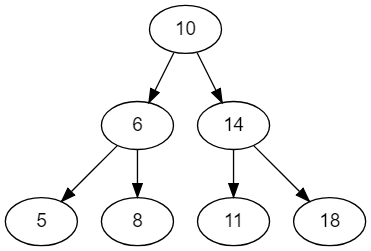
\includegraphics[width=\textwidth]{bst1.png}
    \label{fig:bst1}
    \caption{Δυαδικό δένδρο αναζήτησης}
  \end{minipage}
  \hfill
  \begin{minipage}[b]{0.4\textwidth}
    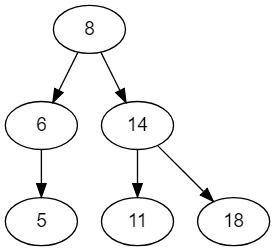
\includegraphics[width=\textwidth]{bst2.png}
    \label{fig:bst2}
    \caption{Το δυαδικό δένδρο αναζήτησης μετά τη διαγραφή της ρίζας}
  \end{minipage}
\end{figure}

\section{Ισοζυγισμένα δυαδικά δένδρα αναζήτησης}
\label{bbst}

Οι καλές επιδόσεις ενός δυαδικού δένδρου αναζήτησης χάνονται όταν το δένδρο δεν είναι ισοζυγισμένο (balanced), δηλαδή όταν υπάρχουν μονοπάτια από τη ρίζα προς τα φύλλα με μεγάλα βάθη ενώ άλλα μονοπάτια έχουν μικρά βάθη. Υπάρχουν διάφορες μορφές ισοζυγισμένων δένδρων με πλέον δημοφιλή τα κόκκινα-μαύρα δένδρα (red black trees) και τα AVL (Adelson, Velskii και Landis) δένδρα. Σε αυτά τα δένδρα πραγματοποιούνται ειδικές λειτουργίες (περιστροφές) έτσι ώστε κατά την εισαγωγή νέων τιμών στο δένδρο και τη διαγραφή τιμών από το δένδρο, τα βάθη των φύλλων του δένδρου εγγυημένα να διατηρούνται σε κοντινές τιμές μεταξύ τους. Ισχύει ότι τα AVL δένδρα είναι καλύτερα ισοζυγισμένα από τα κόκκινα-μαύρα δένδρα αλλά έχουν το μειονέκτημα της υψηλότερης υπολογιστικής επιβάρυνσης κατά την εισαγωγή και τη διαγραφή κόμβων.

\section{Παραδείγματα}

\subsection{Παράδειγμα 1}

Δεδομένου ενός δυαδικού δένδρου ζητείται η εκτύπωση όλων των διαδρομών από τη ρίζα του δένδρου μέχρι κάθε φύλλο. Για παράδειγμα, για το δένδρο του Σχήματος~\ref{fig:binary_tree1} το πρόγραμμα θα πρέπει να επιστρέψει ABDH, ABE, ACF και ACG.

\lstinputlisting[caption = Λύση παραδείγματος 1 (lab09\_ex1.cpp)]{lab09/lab09_ex1.cpp}

Η μεταγλώττιση και η εκτέλεση του κώδικα γίνεται με τις ακόλουθες εντολές:

\lstinputlisting[style=DOS]{lab09/compile_execute3.txt}

Η δε έξοδος που παράγεται είναι η ακόλουθη:

\lstinputlisting[style=DOS]{lab09/lab09_ex1.out}


\subsection{Παράδειγμα 2}

Δεδομένου ενός δυαδικού δένδρου ζητείται να πραγματοποιείται έλεγχος σχετικά με το εάν το δένδρο είναι δυαδικό δένδρο αναζήτησης ή όχι. 

\section{Ασκήσεις}

\begin{enumerate}
\item Να γράψετε πρόγραμμα που να εμφανίζει τους κόμβους ενός δυαδικού δένδρου κατά επίπεδα από κάτω προς τα πάνω και από αριστερά προς τα δεξιά. Δηλαδή στο δένδρο του Σχήματος \ref{fig:binary_tree1} θα πρέπει οι κόμβοι να εμφανιστούν ως D,E,F,G,B,C,A.
\item Να γράψετε πρόγραμμα που να δημιουργεί από έναν ταξινομημένο πίνακα ακεραίων ένα δυαδικό δένδρο αναζήτησης. Να χρησιμοποιηθεί ο ακόλουθος αλγόριθμος:
	\begin{enumerate}
	\item Εύρεση του μεσαίου στοιχείου του πίνακα και ορισμός του ως ρίζα του δένδρου
	\item Αναδρομική εκτέλεση για το αριστερό και το δεξιό μισό
		\begin{enumerate}
		\item Εύρεση του μεσαίου στοιχείου του αριστερού μέρους και ορισμός του ως 		αριστερό παιδί της ρίζας του βήματος α'
		\item Εύρεση του μεσαίου στοιχείου του δεξιού μέρους και ορισμός του ως δεξί παιδί της ρίζας του βήματος α'
		\end{enumerate}
	\end{enumerate}
\end{enumerate}

\begin{thebibliography}{9}
\bibitem{wikipedia_binary_tree}
Wikipedia, Tree (data structure), \href{https://en.wikipedia.org/wiki/Tree_(data_structure)}{https://en.wikipedia.org/wiki/Tree\_(data\_structure)}

\bibitem{parlante_binary_tree}
Binary Trees by Nick Parlante, \href{http://cslibrary.stanford.edu/110/BinaryTrees.html}{http://cslibrary.stanford.edu/110/BinaryTrees.html}

\bibitem{wikipedia_polish_notation}
Wikipedia, Polish Notation, \href{https://en.wikipedia.org/wiki/Polish_notation}{https://en.wikipedia.org/wiki/Polish\_notation}

\bibitem{wikipedia_reverse_polish_notation}
Wikipedia, Reverse Polish Notation, \href{https://en.wikipedia.org/wiki/Reverse_Polish_notation}{https://en.wikipedia.org/wiki/Reverse\_Polish\_notation}

\bibitem{g4g_traversals}
Tree Traversals (Inorder, Preorder and Postorder), \href{https://www.geeksforgeeks.org/tree-traversals-inorder-preorder-and-postorder/}{https://www.geeksforgeeks.org/tree-traversals-inorder-preorder-and-postorder/}

\bibitem{jumping_into_cpp}
Alex Allain, Jumping into C++, cprogramming.com, Chapter 17 - Binary Trees, 2013

\end{thebibliography}

